% 注意事项:编译两次,以确保目录、页码完整显示

\def\allfiles{}

\documentclass[14pt,a4paper,UTF8,twoside]{article}

% Formatting Packages ——————————————————————————————————————
\usepackage{multicol}
\usepackage{multirow}
\usepackage{enumitem}
\usepackage{indentfirst}
\usepackage[toc]{multitoc}

% Math & Physics Packages ————————————————————————————
\usepackage{amsmath, amsthm, amsfonts, amssymb}
\usepackage{setspace}
\usepackage{physics}
\usepackage{cancel}
\usepackage{nicefrac}
\usepackage{unicode-math} % 允许数学公式使用特定字体

% Image-related Packages —————————————————————————————
\usepackage{float} % 浮动体环境
\usepackage{subcaption} % 子图包
\usepackage{graphics, graphicx}
\usepackage{tikz, tikz-qtree}
\usetikzlibrary{arrows.meta}
\usetikzlibrary{shapes.geometric, arrows}
\tikzstyle{node_style} = [rectangle, rounded corners, draw, align=center, text width=3cm, minimum height=0.65cm]
\tikzstyle{arrow_style} = [thick, ->, >=stealth]

\usepackage{pgfplots}
\pgfplotsset{compat=1.18}
\usepackage{xcolor}
\usepackage{fourier-orns}
\usepackage{lipsum}

% Colour Palette ——————————————————————————————————————
\definecolor{merah}{HTML}{F4564E}
\definecolor{merahtua}{HTML}{89313E}
\definecolor{biru}{HTML}{60BBE5}
\definecolor{birutua}{HTML}{412F66}
\definecolor{hijau}{HTML}{59CC78}
\definecolor{hijautua}{HTML}{366D5B}
\definecolor{kuning}{HTML}{FFD56B}
\definecolor{jingga}{HTML}{FBA15F}
\definecolor{ungu}{HTML}{8C5FBF}
\definecolor{lavender}{HTML}{CBA5E8}
\definecolor{merjamb}{HTML}{FFB6E0}
\definecolor{mygray}{HTML}{E6E6E6}
\definecolor{mygreen}{rgb}{0,0.6,0}
\definecolor{mymauve}{rgb}{0.58,0,0.82}

% Theorems ————————————————————————————————————————————
\usepackage{tcolorbox}
\usepackage{changepage}
\tcbuselibrary{skins,breakable,theorems}

\newcounter{hitung}
\setcounter{hitung}{\thesection}

\makeatletter
	% Proof 证明如下
	\def\tcb@theo@widetitle#1#2#3{\hbox to \textwidth{\textsc{\large#1}\normalsize\space#3\hfil(#2)}}
	\tcbset{
		theorem style/theorem wide name and number/.code={ \let\tcb@theo@title=\tcb@theo@widetitle},
		proofbox/.style={skin=enhancedmiddle,breakable,parbox=false,boxrule=0mm,
			check odd page, toggle left and right, colframe=black!20!white!92!hijau,
			leftrule=8pt, rightrule=0mm, boxsep=0mm,arc=0mm, outer arc=0mm,
			left=3mm,right=3mm,top=0mm,bottom=0mm, toptitle=0mm,
			bottomtitle=0mm,colback=gray!3!white!98!biru, before skip=8pt, after skip=8pt,
			before={\par\vskip-2pt},after={\par\smallbreak},
		},
	}
	\newtcolorbox{ProofBox}{proofbox}
	\makeatother
	
	\let\realproof\proof
	\let\realendproof\endproof
	\renewenvironment{proof}[1][Prove:]{\ProofBox\strut\textsc{#1}\space}{\endProofBox}
        \AtEndEnvironment{proof}{\null\hfill$\blacksquare$}
        % Definition 定义环境
	\newtcbtheorem[use counter=hitung, number within=section]{dfn}{定义}
	{theorem style=theorem wide name and number,breakable,enhanced,arc=3.5mm,outer arc=3.5mm,
		boxrule=0pt,toprule=1pt,leftrule=0pt,bottomrule=1pt, rightrule=0pt,left=0.2cm,right=0.2cm,
		titlerule=0.5em,toptitle=0.1cm,bottomtitle=-0.1cm,top=0.2cm,
		colframe=white!10!biru,
		colback=white!90!biru,
		coltitle=white,
		shadow={1.3mm}{-1.3mm}{0mm}{gray!50!white}, % 添加阴影
        coltext=birutua!60!gray, title style={white!10!biru}, rbefoe skip=8pt, after skip=8pt,
		fonttitle=\bfseries,fontupper=\normalsize}{dfn}

	% 答题卡
	\newtcbtheorem[use counter=hitung, number within=section]{ans}{解答}
	{theorem style=theorem wide name and number,breakable,enhanced,arc=3.5mm,outer arc=3.5mm,
		boxrule=0pt,toprule=1pt,leftrule=0pt,bottomrule=1pt, rightrule=0pt,left=0.2cm,right=0.2cm,
		titlerule=0.5em,toptitle=0.1cm,bottomtitle=-0.1cm,top=0.2cm,
		colframe=white!10!biru,
		colback=white!90!biru,
		coltitle=white,
		shadow={1.3mm}{-1.3mm}{0mm}{gray!50!white}, % 添加阴影
        coltext=birutua!60!gray, title style={white!10!biru}, before skip=8pt, after skip=8pt,
		fonttitle=\bfseries,fontupper=\normalsize}{ans}

	% Axiom
	\newtcbtheorem[use counter=hitung, number within=section]{axm}{公理}
	{theorem style=theorem wide name and number,breakable,enhanced,arc=3.5mm,outer arc=3.5mm,
		boxrule=0pt,toprule=1pt,leftrule=0pt,bottomrule=1pt, rightrule=0pt,left=0.2cm,right=0.2cm,
		titlerule=0.5em,toptitle=0.1cm,bottomtitle=-0.1cm,top=0.2cm,
		colframe=white!10!biru,colback=white!90!biru,coltitle=white,
		shadow={1.3mm}{-1.3mm}{0mm}{gray!50!white!90}, % 添加阴影
        coltext=birutua!60!gray,title style={white!10!biru},before skip=8pt, after skip=8pt,
		fonttitle=\bfseries,fontupper=\normalsize}{axm}
 
	% Theorem
	\newtcbtheorem[use counter=hitung, number within=section]{thm}{定理}
	{theorem style=theorem wide name and number,breakable,enhanced,arc=3.5mm,outer arc=3.5mm,
		boxrule=0pt,toprule=1pt,leftrule=0pt,bottomrule=1pt, rightrule=0pt,left=0.2cm,right=0.2cm,
		titlerule=0.5em,toptitle=0.1cm,bottomtitle=-0.1cm,top=0.2cm,
		colframe=white!10!merah,colback=white!75!pink,coltitle=white, coltext=merahtua!80!merah,
		shadow={1.3mm}{-1.3mm}{0mm}{gray!50!white!90}, % 添加阴影
		title style={white!10!merah}, before skip=8pt, after skip=8pt,
		fonttitle=\bfseries,fontupper=\normalsize}{thm}
	
	% Proposition
	\newtcbtheorem[use counter=hitung, number within=section]{prp}{命题}
	{theorem style=theorem wide name and number,breakable,enhanced,arc=3.5mm,outer arc=3.5mm,
		boxrule=0pt,toprule=1pt,leftrule=0pt,bottomrule=1pt, rightrule=0pt,left=0.2cm,right=0.2cm,
		titlerule=0.5em,toptitle=0.1cm,bottomtitle=-0.1cm,top=0.2cm,
		colframe=white!10!hijau,colback=white!90!hijau,coltitle=white, coltext=hijautua!80!brown,
		shadow={1.3mm}{-1.3mm}{0mm}{gray!50!white}, % 添加阴影
		title style={white!10!hijau}, before skip=8pt, after skip=8pt,
		fonttitle=\bfseries,fontupper=\normalsize}{prp}


	% Example
	\newtcolorbox[use counter=hitung, number within=section]{cth}[1][]{breakable,
		colframe=white!10!jingga, coltitle=white!90!jingga, colback=white!85!jingga, coltext=black!10!brown!50!jingga, colbacktitle=white!10!jingga, enhanced, fonttitle=\bfseries,fontupper=\normalsize, attach boxed title to top left={yshift=-2mm}, before skip=8pt, after skip=8pt,
		title=Contoh~\thetcbcounter \ \ #1}

	% Catatan/Note
	\newtcolorbox{ctt}[1][]{enhanced, 
		left=4.1mm, borderline west={8pt}{0pt}{white!10!kuning}, 
		before skip=6pt, after skip=6pt, 
		colback=white!85!kuning, colframe= white!85!kuning, coltitle=orange!60!kuning!25!brown, coltext=orange!60!kuning!25!brown,
		fonttitle=\bfseries,fontupper=\normalsize, before skip=8pt, after skip=8pt,
		title=\underline{Catatan}  #1}
	
	% Komentar/Remark
	\newtcolorbox{rmr}[1][]{
		,arc=0mm,outer arc=0mm,
		boxrule=0pt,toprule=1pt,leftrule=0pt,bottomrule=5pt, rightrule=0pt,left=0.2cm,right=0.2cm,
		titlerule=0.5em,toptitle=0.1cm,bottomtitle=-0.1cm,top=0.2cm,
		colframe=white!10!kuning,colback=white!85!kuning,coltitle=white, coltext=orange!60!kuning,
		fonttitle=\bfseries,fontupper=\normalsize, before skip=8pt, after skip=8pt,
		title=Komentar  #1}

\usepackage{booktabs} % 表格库
\usepackage{titlesec} % 标题库
\usepackage{fancyhdr} % 页眉页脚库
\usepackage[sorting=none]{biblatex}
\usepackage{array}
\addbibresource{references.bib} % 指定你的.bib文件名称

\date{} % 留空,以让编译时去除日期

%———————————————注意事项—————————————————%

% 1、如果编译显示失败,但没有错误信息,就是 filename.pdf 正在被占用
% 2、在文件夹中的终端使用 Windows > xelatex filename.tex 也可编译

%—————————————华东师范大学———————————————%

% 论文制作时须加页眉,页眉从中文摘要开始至论文末
% 偶数页码内容为:华东师范大学硕士学位论文,奇数页码内容为学位论文题目

%————————定义 \section 的标题样式————————%

% 注意:\chapter 等命令,内部使用的是 \thispagestyle{plain} 的排版格式
% 若需要自己加上页眉,实际是在用 \thispagestyle{fancy} 的排版格式
% 加上下面这一段指令,就能够让 \section 也使用 fancy 的排版格式
% 本质就是让目录、第一页也能够显示页眉、页脚

\fancypagestyle{plain}{
  \pagestyle{fancy}
}

\title{华东师范大学软件学院实验报告} % 模板
\titleformat{\section}
    {\normalfont\bfseries\Large} % 字体大小、字体系列(\bfseries 为加粗)
    {\thesection}{1em}{}

% ———————————设置章节的中文格式———————————%
\renewcommand\thesection{\chinese{section} \hspace{0pt}}
\renewcommand\thesubsection{\arabic{subsection} \hspace{0pt}}
% \renewcommand\thesubsubsection{\alph{subsubsection} \hspace{0pt}} % 字母编号
% \hspace{0pt} 是为了确保在章节编号和章节题目之间不要有空格,使得排版更为美观
    
%—————————————页面基础设置———————————————%

\usepackage{geometry}
\geometry{left=10mm, right=10mm, top=20mm, bottom=20mm}

%————————————设置页眉、页脚——————————————%

\pagestyle{fancy} % 设置 plain style 的属性

% 设置页眉

\fancyhead[RE]{\leftmark} % Right Even 偶数页右侧显示章名 \leftmark 最高级别章名
\fancyhead[LO]{\rightmark} % Left Odd 奇数页左侧显示节名 \rightmark 第二级别节名
\fancyhead[C]{华东师范大学软件学院实验报告} % Center 居中显示
\fancyhead[LE,RO]{~\thepage~} % 在偶数页的左侧,奇数页的右侧显示页码
\renewcommand{\headrulewidth}{1.2pt} % 页眉与正文之间的水平线粗细

% 设置页脚:在每页的右下脚以斜体显示书名

\fancyfoot[RO,RE]{\it Lab Report By \LaTeX} % 使用意大利斜体显示
\renewcommand{\footrulewidth}{0.5pt} % 页脚水平线宽度

%——————设置页码:在底部居中显示页码———————%

\usepackage{lastpage} % 页码数库
\pagestyle{fancy}
\fancyfoot[C]{\kaishu 第 \thepage 页 \ 共 \pageref{LastPage} 页} % LastPage 需要二次编译以获取总页数

%——————————————代码块设置———————————————%

\usepackage{listings} % 代码块包
\lstset {
    backgroundcolor=\color{white},   % choose the background color; you must add \usepackage{color} or \usepackage{xcolor}
    basicstyle=\footnotesize,        % the size of the fonts that are used for the code
    breakatwhitespace=false,         % sets if automatic breaks should only happen at whitespace
    breaklines=true,                 % sets automatic line breaking
    captionpos=bl,                   % sets the caption-position to bottom
    commentstyle=\color{mygreen},    % comment style
    deletekeywords={...},            % if you want to delete keywords from the given language
    escapeinside={\%*}{*},           % if you want to add LaTeX within your code
    extendedchars=true,              % lets you use non-ASCII characters; for 8-bits encodings only, does not work with UTF-8
    frame=single,                    % adds a frame around the code
    keepspaces=true,                 % keeps spaces in text, useful for keeping indentation of code (possibly needs columns=flexible)
    keywordstyle=\color{blue},       % keyword style
    % language=Python,               % the language of the code
    morekeywords={*,...},            % if you want to add more keywords to the set
    numbers=left,                    % where to put the line-numbers; possible values are (none, left, right)
    numbersep=5pt,                   % how far the line-numbers are from the code
    numberstyle=\tiny\color{mygray}, % the style that is used for the line-numbers
    rulecolor=\color{black},         % if not set, the frame-color may be changed on line-breaks within not-black text (e.g. comments (green here))
    showspaces=false,                % show spaces everywhere adding particular underscores; it overrides 'showstringspaces'
    showstringspaces=false,          % underline spaces within strings only
    showtabs=false,                  % show tabs within strings adding particular underscores
    stepnumber=1,                    % the step between two line-numbers. If it's 1, each line will be numbered
    stringstyle=\color{orange},      % string literal style
    tabsize=2,                       % sets default tabsize to 2 spaces
    % title=Python Code              % show the filename of files included with \lstinputlisting; also try caption instead of title
}

% 注释掉的部分用于后续插入代码,参数可调整,格式如下:

% 1、直接插入
% \begin{lstlisting}[language = ? , title = { ? } ]
%       Your code here.
% \end{lstlisting}

% 2、文件插入
% \lstinputlisting[language = C , title = ?.c] {filename.c}

%———————————————字体设置————————————————%

\usepackage{fontspec} % 允许设置字体
\usepackage[utf8]{inputenc}
\usepackage{ctex}
\linespread{1.2}
% \setCJKmainfont{SimSun} % 设置正文罗马族的 CJK 字体

%———————————————超链接设置——————————————%

\usepackage[hidelinks]{hyperref}
\hypersetup{
    pdfstartview=FitH, % 设置PDF文档打开时的初始视图为页面宽度适应窗口宽度(即页面水平适应)
    CJKbookmarks=true, % 用对CJK(中文、日文、韩文)字符的书签支持,确保这些字符在书签中正确显示
    bookmarksnumbered=true, % 书签带有章节编号。这对有章节编号的文档很有用
    bookmarksopen=true, % 文档打开时,书签树是展开的,方便查看所有书签
    colorlinks, % 启用彩色链接。这样,链接在PDF中会显示为彩色,而不是默认的方框
    pdfborder=001, % 设置PDF文档中链接的边框样式。001 表示链接周围没有边框,仅在单击时显示一个矩形
    linkcolor=blue, % 设置文档内部链接(如目录中的章节链接)的颜色为蓝色
    anchorcolor=blue, % 设置锚点链接(即目标在同一文档内的链接)的颜色为蓝色
    citecolor=blue, % 设置引用(如文献引用)的颜色为蓝色
}

%————————————导言区结束,进入正文部分————————————%

\begin{document}

\maketitle

\begin{center} % \extracolsep{\fill} 拉伸到页面最大宽度前,保证居中显示

  \begin{tabular*}{\textwidth}{@{\extracolsep{\fill}} l  l  l }
    \hline
    实验课程:计算机网络实践 &  年级:2023级本科  &  实验成绩: \\
    实验名称:Lab 3 IPv4 & 姓名:张梓卫 \\
    实验编号:(3) & 学号:10235101526 & 实验日期:2024/12/06 \\
    指导老师:刘献忠 & 组号:& 实验时间:2 课时 \\
    \hline
  \end{tabular*}

\end{center}

\tableofcontents % 目录也需要二次编译

\section{实验目的}

该实验是课程《计算机网络实践》的第三次实验,全名《IPV4》,目标如下:

\begin{itemize}
    \item 1. 学会通过Wireshark分析ip协议
    \item 2. 了解IP数据报的组成
    \item 3. 了解IP各部分的含义    
\end{itemize}

\section{实验内容与实验步骤}

\begin{itemize}
    \item 启动Wireshark,在菜单栏的捕获->选项中进行设置
    \item 选择已连接的以太网,设置捕获过滤器为“tcp port 80”,将混杂模式设为关闭
    \item 勾选 enable network name resolution.然后开始捕获。
    \item 打开windows的命令行,在里面输入wget www.sina.com
    \item 打开Wireshark,停止捕获。    
\end{itemize}

\section{实验环境}

使用 Wireshark v4.2.5, Windows 11 Pro, Wget Tools 进行实验。

实验报告使用 \LaTeX 进行撰写,使用 Vim 编辑器进行文本编辑。

\section{实验过程与分析}

\subsection{获取 IP Packets}

\subsubsection{启动 Wireshark 捕获数据包}

启动 Wireshark,按照实验要求将捕获选项设置为:已连接的以太网,设置捕获过滤器为 tcp port 80,将混杂模式设为关闭,勾选 enable network name resolution。

\begin{figure}[H]
  \centering
  \includegraphics[width=0.6\textwidth]{lab3/fitler.jpg}
  \caption{Wireshark Filter}
\end{figure}

设置 rename 选项为开启:

\begin{figure}[H]
  \centering
  \includegraphics[width=0.4\textwidth]{lab3/rename.png}
  \caption{Wireshark Rename}
\end{figure}

\subsubsection{使用 Wget 命令}

打开命令行,输入:\texttt{wget www.sina.com}

\begin{figure}[H]
  \centering
  \includegraphics[width=0.6\textwidth]{lab3/wget.png}
  \caption{Wget Command}
\end{figure}

\subsubsection{停止捕获}

根据命令行显示,\href{www.sina.com}{www.sina.com} 的主机地址为 61.170.80.226,在 Wireshark 捕获数据包。

\begin{figure}[H]
  \centering
  \includegraphics[width=0.6\textwidth]{lab3/get.png}
  \caption{Get}
\end{figure}

\subsubsection{使用 Tracert 追踪路径信息}

在 Windows 中,Tracert 命令是直接使用 \texttt{Tracert www.sina.com} 即可进行跃点跟踪路由。

使用命令后,等待一段时间,结果如下:

\begin{figure}[H]
  \centering
  \includegraphics[width=0.5\textwidth]{lab3/tracert.png}
  \caption{Tracert}
\end{figure}

\subsubsection{IP 报文的结构}

接下来查看 Wireshark 抓包获取的信息,左右两边结合为一张图片,如下图所示:

\begin{figure}[H]
  \centering
  \includegraphics[width=0.7\textwidth]{lab3/combina.jpg}
  \caption{Combination}
\end{figure}

根据 Wireshark 内的提示以及课件上的信息,我先给图中的字节进行信息标注:

\begin{figure}[H]
  \centering
  \includegraphics[width=0.8\textwidth]{lab3/result.jpg}
  \caption{Bites in Pic}
\end{figure}

对齐填充后,得到如下的 IP 报文结构,注意这里是从远程计算机发送至本地计算机的抓包:

\section*{对齐整理:}

\begin{center}
\setlength{\extrarowheight}{2pt}
\begin{tabular}{|c|c|c|c|}
\hline
Version (4 bit) & IHL (4 bit) & Type of Service (8 bit) & Total Length (16 bit) \\ 
\hline
Identification (16 bit) & \multicolumn{2}{c|}{Flags (3 bit)} & Fragment Offset (13 bit) \\ 
\hline
Time To Live (8 bit) & Protocol (8 bit) & \multicolumn{2}{c|}{Header Checksum (16 bit)} \\ 
\hline
\multicolumn{4}{|c|}{Source IP Address (32 bit)} \\ 
\hline
\multicolumn{4}{|c|}{Destination IP Address (32 bit)} \\ 
\hline
\multicolumn{2}{|c|}{Options (variable)} & \multicolumn{2}{c|}{Padding (variable)} \\ 
\hline
\end{tabular}
\end{center}

\subsubsection{回答问题}
由于我选取的抓包示例是从远程计算机发送至本地计算机的,对于实验手册中的问题,我的回答如下:

1.What are the IP addresses of your computer and the remote server?

查看 Source Address 和 Destination Address,分别为:

\begin{lstlisting}
Source Address: 61.170.80.226 # 远程服务器的 IP 地址
Destination Address: 192.168.1.114 # 本地计算机的 IP 地址
\end{lstlisting}

\vspace{0.5cm}

2. Does the Total Length field include the IP header plus IP payload, or just the IP payload?

根据 IP 报文结构,我们可以知道,总长度包含了 IP 协议头 和 IP 的有效负载,这在 Wireshark 中是显然的。

\vspace{0.5cm}

3. How does the value of the Identification field change or stay the same for different packets? 
For instance, does it hold the same value for all packets in a TCP connection or does it differ 
for each packet? Is it the same in both directions? Can you see any pattern if the value does 
change?

不同的数据包具有不同的标识字段,但若是不分段,则Identification为0x0000。每个报文的Identification字段一般来说不相同。
IP软件在存储器中维持一个计数器,每产生一个数据报,计数器就加1,并将此值赋给标识字段。
但这个“标识”不是序号,因为IP是无连接服务,数据报不存在按序接收的问题。当数据报由于长度超过网络的MTU而必须分片时,
这个标识字段的值就被复制到所有的数据报片的标识字段中。相同的标识字段的值使分片后的各数据报片最后能正确地重装成为原来的数据报。

识别字段在双向通信中通常是不同的。每个数据包的识别字段是由发送方独立设置的。由于源主机和目标主机的 IP 栈是独立运行的,从 主机 A 到主机 B 的数据包的识别字段通常会有一个序列,而从 主机 B 到主机 A 的数据包会有不同的序列。

识别字段的变化是有一定模式的:

顺序递增:大多数系统会为每个发送的数据包顺序递增识别字段的值。例如,如果第一个数据包的 ID 是 1000,那么下一个数据包可能是 1001,以此类推。这在 IPv4 中尤其常见。
一些操作系统或配置(例如某些 Linux 设置)会将识别字段设置为随机值,以避免可预测性,尤其是在设置了 不可分片(DF) 位时。这种情况下,可能会使得模式不容易观察到。
如果设置了 不可分片(DF) 位,并且数据包没有被分片,则识别字段可能在一些实现中保持恒定。

\vspace{0.5cm}

4. What is the initial value of the TTL field for packets sent from your computer? Is it the 
maximum possible value, or some lower value?

在我的 Wireshark 抓包中,从个人计算机 (192.168.1.114) 发送的 IP 报文的 TTL 字段初始值为 128,这里应该点开 Source Address 为 61.170.80.226 的 IP 报文,查看 TTL 字段的值。

\begin{figure}[H]
  \centering
  \includegraphics[width=0.6\textwidth]{lab3/ttl.png}
  \caption{TTL}
\end{figure}

\vspace{0.5cm}

5. How can you tell from looking at a packet that it has not been fragmented? Most often IP 
pack- ets in normal operation are not fragmented. But the receiver must have a way to be sure. 
Hint: you may need to read your text to confirm a guess.

只需要观察 Wireshark 中的 Don't Fragment 位是否被置为了 1 即可。

\begin{figure}[H]
\centering
  \includegraphics[width=0.45\textwidth]{lab3/fragment.png}
  \caption{Don't Fragment}
\end{figure}

\vspace{0.5cm}

6. What is the length of the IP Header and how is this encoded in the header length field? Hint:
notice that only 4 bits are used for this field, as the version takes up the other 4 bits of the 
byte. You may guess and check your text.

IP 协议头的第 5-8 位 Header Length 即为协议头的长度。这 4 位的十进制值域为 5-15,
5 代表没有额外可选的协议头,即长度为 20 字节;为 15 为最大长度,最多为 60 字
节。故头部长度范围为 20 字节到 60 字节。

\begin{figure}[H]
  \centering
  \includegraphics[width=0.6\textwidth]{lab3/IHL.png}
  \caption{Header Length}
\end{figure}

\subsection{Step 4: Internet Paths}

之前获取到的 tracert 路径如下图所示:

\begin{figure}[H]
  \centering
  \includegraphics[width=0.6\textwidth]{lab3/tracert.png}
  \caption{Tracert}
\end{figure}

\begin{center}
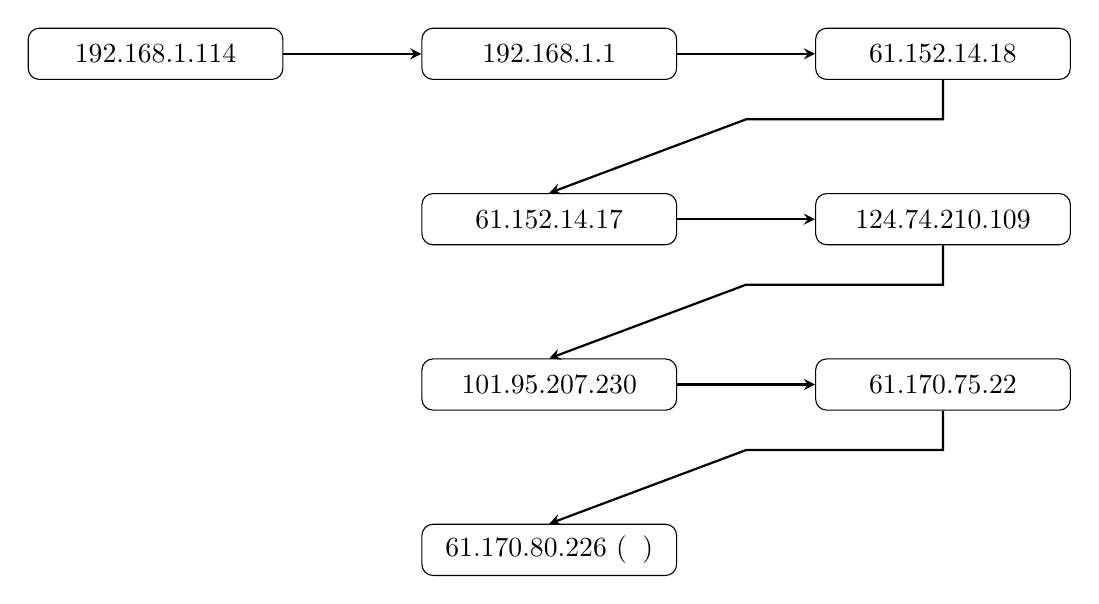
\begin{tikzpicture}[node distance=2cm and 3cm]

  % 第一行
  \node[node_style] (node0) {192.168.1.114}; % 新增节点
  \node[node_style, right of=node0, xshift=3cm] (node1) {192.168.1.1};
  \node[node_style, right of=node1, xshift=3cm] (node2) {61.152.14.18};
  \draw[arrow_style] (node0.east) -- (node1.west); % 新增连接
  \draw[arrow_style] (node1.east) -- (node2.west);
  
  % 第二行
  \node[node_style, below of=node1, yshift=-0.1cm] (node3) {61.152.14.17};
  \node[node_style, right of=node3, xshift=3cm] (node4) {124.74.210.109};
  \draw[arrow_style] (node2.south) -- ++(0,-0.5) -- ++(-2.5,0) -- (node3.north);
  \draw[arrow_style] (node3.east) -- (node4.west);
  
  % 第三行
  \node[node_style, below of=node3, yshift=-0.1cm] (node5) {101.95.207.230};
  \node[node_style, right of=node5, xshift=3cm] (node6) {61.170.75.22};
  \draw[arrow_style] (node4.south) -- ++(0,-0.5) -- ++(-2.5,0) -- (node5.north);
  \draw[arrow_style] (node5.east) -- (node6.west);
  
  % 第四行
  \node[node_style, below of=node5, yshift=-0.1cm] (node7) {61.170.80.226 (目标)};
  \draw[arrow_style] (node6.south) -- ++(0,-0.5) -- ++(-2.5,0) -- (node7.north);
  
  \end{tikzpicture}
\end{center}

\subsection{Step 5: IP Header Checksum}

根据 PPT 中的帮助说明,计算对IP首部检验和的算法如下:
\begin{itemize}
  \item (1)把IP数据包的校验和字段置为0。
  \item (2)把首部看成以16位为单位的数字组成,依次进行二进制求和(注意:求和时应将最高位的进位保存,所以加法应采用32位加法)。
  \item (3)将上述加法过程中产生的进位(最高位的进位)加到低16位(采用32位加法时,即为将高16位与低16位相加,之后还要把该次加法最高位产生的进位加到低16位)。
  \item (4)将上述的和取反,即得到校验和。
\end{itemize}

先选择一个 IPV4 协议头,查看其 20 字节的字段。

\begin{figure}[H]
  \centering
  \includegraphics[width=0.9\textwidth]{lab3/checksumready.png}
  \caption{Checksum}
\end{figure}

取出这 20 字段,首先把校验和字段置为 0。

\begin{lstlisting}
  45 00 -> 4500
  05 c8 -> 05c8
  d0 0f -> d00f
  40 00 -> 4000
  39 06 -> 3906
  1b 7a -> 0000 # 设置为 0
  3d aa -> 3daa
  50 e2 -> 50e2
  c0 a8 -> c0a8
  01 72 -> 0172  
\end{lstlisting}

然后进行二进制求和,这一部分我使用计算器来完成:

\begin{figure}[H]
  \centering
  \includegraphics[width=0.4\textwidth]{lab3/calculator.png}
  \caption{Checksum}
\end{figure}

\[
E483 + 0002 = E485
\]

之后,使用按位取反功能,完成最后一步 Checksum 的计算。

\begin{figure}[H]
  \centering
  \includegraphics[width=0.4\textwidth]{lab3/NOT.png}
  \caption{NOT}
\end{figure}

\textbf{这与 Wireshark 中的校验和一致:}

\begin{figure}[H]
  \centering
  \includegraphics[width=0.8\textwidth]{lab3/check.png}
  \caption{The same checksum}
\end{figure}

\subsection{课后思考题}

\subsubsection{IPV6}

现在这个 IPv6 即将普及的时代,它已经不稀有了,在家捣鼓串流时就曾想过用公网 IPv6 来做一些便利性的操作。

在寝室的宿舍网络下,路由器并没有支持 IPv6 的连接,而直接打开 \texttt{ipconfig} 看到的 FE80 实际上就和 192.168 没有什么区别,就是一个局域网内分配的地址而已。

我尝试了使用 ISATAP 隧道来建立 IPV4 与 IPV6 的桥梁,可惜失败了。

我使用的代码为:

\begin{lstlisting}
  netsh interface ipv6 isatap set router isatap.tsinghua.edu.cn
  netsh interface ipv6 isatap set state endabled
  netsh interface ipv6 isatap show state
  >>> enabled
  ping -6 ipv6.google.com
  >>> 无法解析域名
\end{lstlisting}

\begin{figure}[H]
  \centering
  \includegraphics[width=0.6\textwidth]{lab3/isatap.png}
  \caption{ISATAP}
  \label{fig:isatap}
\end{figure}

\subsubsection{隧道协议}

这是一种基于 tunnels 的技术,即把原始的 IP 包封装在另一个数据包内进行传输。

具体的协议包括 IPsec、SSH、Sock 等,它可以用于跨网络通信(如 IPV4 和 IPV6 之间的过渡),还可以提高安全性,实现私有网络和公共网络的互通。
隧道协议的核心工作原理如下:

\begin{enumerate}
  \item 封装:将原始 IP 包作为有效负载,嵌入到一个新数据包中,新数据包会添加一个外层 IP 头部。
  \item 传输:通过隧道协议将封装后的数据包从一个网络节点传输到另一个节点。
  \item 解封装:在目标节点处解封装数据包,提取出原始的 IP 包,并将其转发到最终的目的地。
\end{enumerate}


\subsubsection{IP 安全}

不同的 IP 地址被分配给不同的地区、机构,因此利用公网 IP 能够获取一定的地
理信息知识。

IPsec(IP Security)是IETF制定的三层隧道加密协议,它为Internet上传输的数据提供了高质量的、可互操作的、基于密码学的安全保证。

\begin{enumerate}
  \item 数据机密性(Confidentiality):IPsec发送方在通过网络传输包前对包进行加密。
  \item 数据完整性(Data Integrity):IPsec接收方对发送方发送来的包进行认证,以确保数据在传输过程中没有被篡改。
  \item 数据来源认证(Data Authentication):IPsec在接收端可以认证发送的IPsec报文的发送端是否合法。
  \item 防重放(Anti-Replay):IPsec接收方可检测并拒绝接收过时或重复的报文。
\end{enumerate}

\section{实验结果总结}

通过本次实验,我对IP协议的组成、解析方法及其相关网络协议有了更深入的理解,并熟练掌握了Wireshark抓包工具的使用方法。

实验详细研究了IPv4协议的头部结构,通过实际抓取IP数据包并标注各字段(如版本、头长度、总长度、标识字段等),加深了对IP报文组成部分的认知。
这种对细节的深入解析,让我在理论知识上有了更扎实的积累。
在分析过程中,我结合实际网络行为(如访问新浪网站),通过可视化界面和协议分解信息,验证了IP报文中校验和、TTL等关键字段的计算方法。
在实验中,我研究了IP协议的头部校验和的计算方法,验证了Wireshark中校验和的正确性。同时,我通过tracert命令追踪数据包的网络路径,深入理解了IP分片、跳数限制(TTL)的作用,以及数据包在网络中的传输过程。

\section{附录}

\subsection*{参考资料}

\begin{itemize}
  \item 隧道协议:\href{https://blog.csdn.net/wangjianno2/article/details/75208036}{\underline{https://blog.csdn.net/wangjianno2/article/details/75208036}}
  \item IPv6:\href{https://jingyan.baidu.com/article/22fe7ced67c9443002617f94.html}{\underline{https://jingyan.baidu.com/article/22fe7ced67c9443002617f94.html}}
  \item IP 地址查询:\href{https://www.chaipip.com/ip.php}{\underline{https://www.chaipip.com/ip.php}}
  \item 查询本机 IP:\href{https://ip.cn/}{\underline{https://ip.cn/}}
\end{itemize}

\end{document}